\documentclass[border=10pt]{standalone}
\usepackage[svgnames]{xcolor}
\usepackage{amsmath}
\usepackage{pgfplots}
\pgfplotsset{compat=newest}
\usepackage[sfdefault]{FiraSans}
\usepackage{FiraMono}
\renewcommand*\familydefault{\sfdefault}
\begin{document}
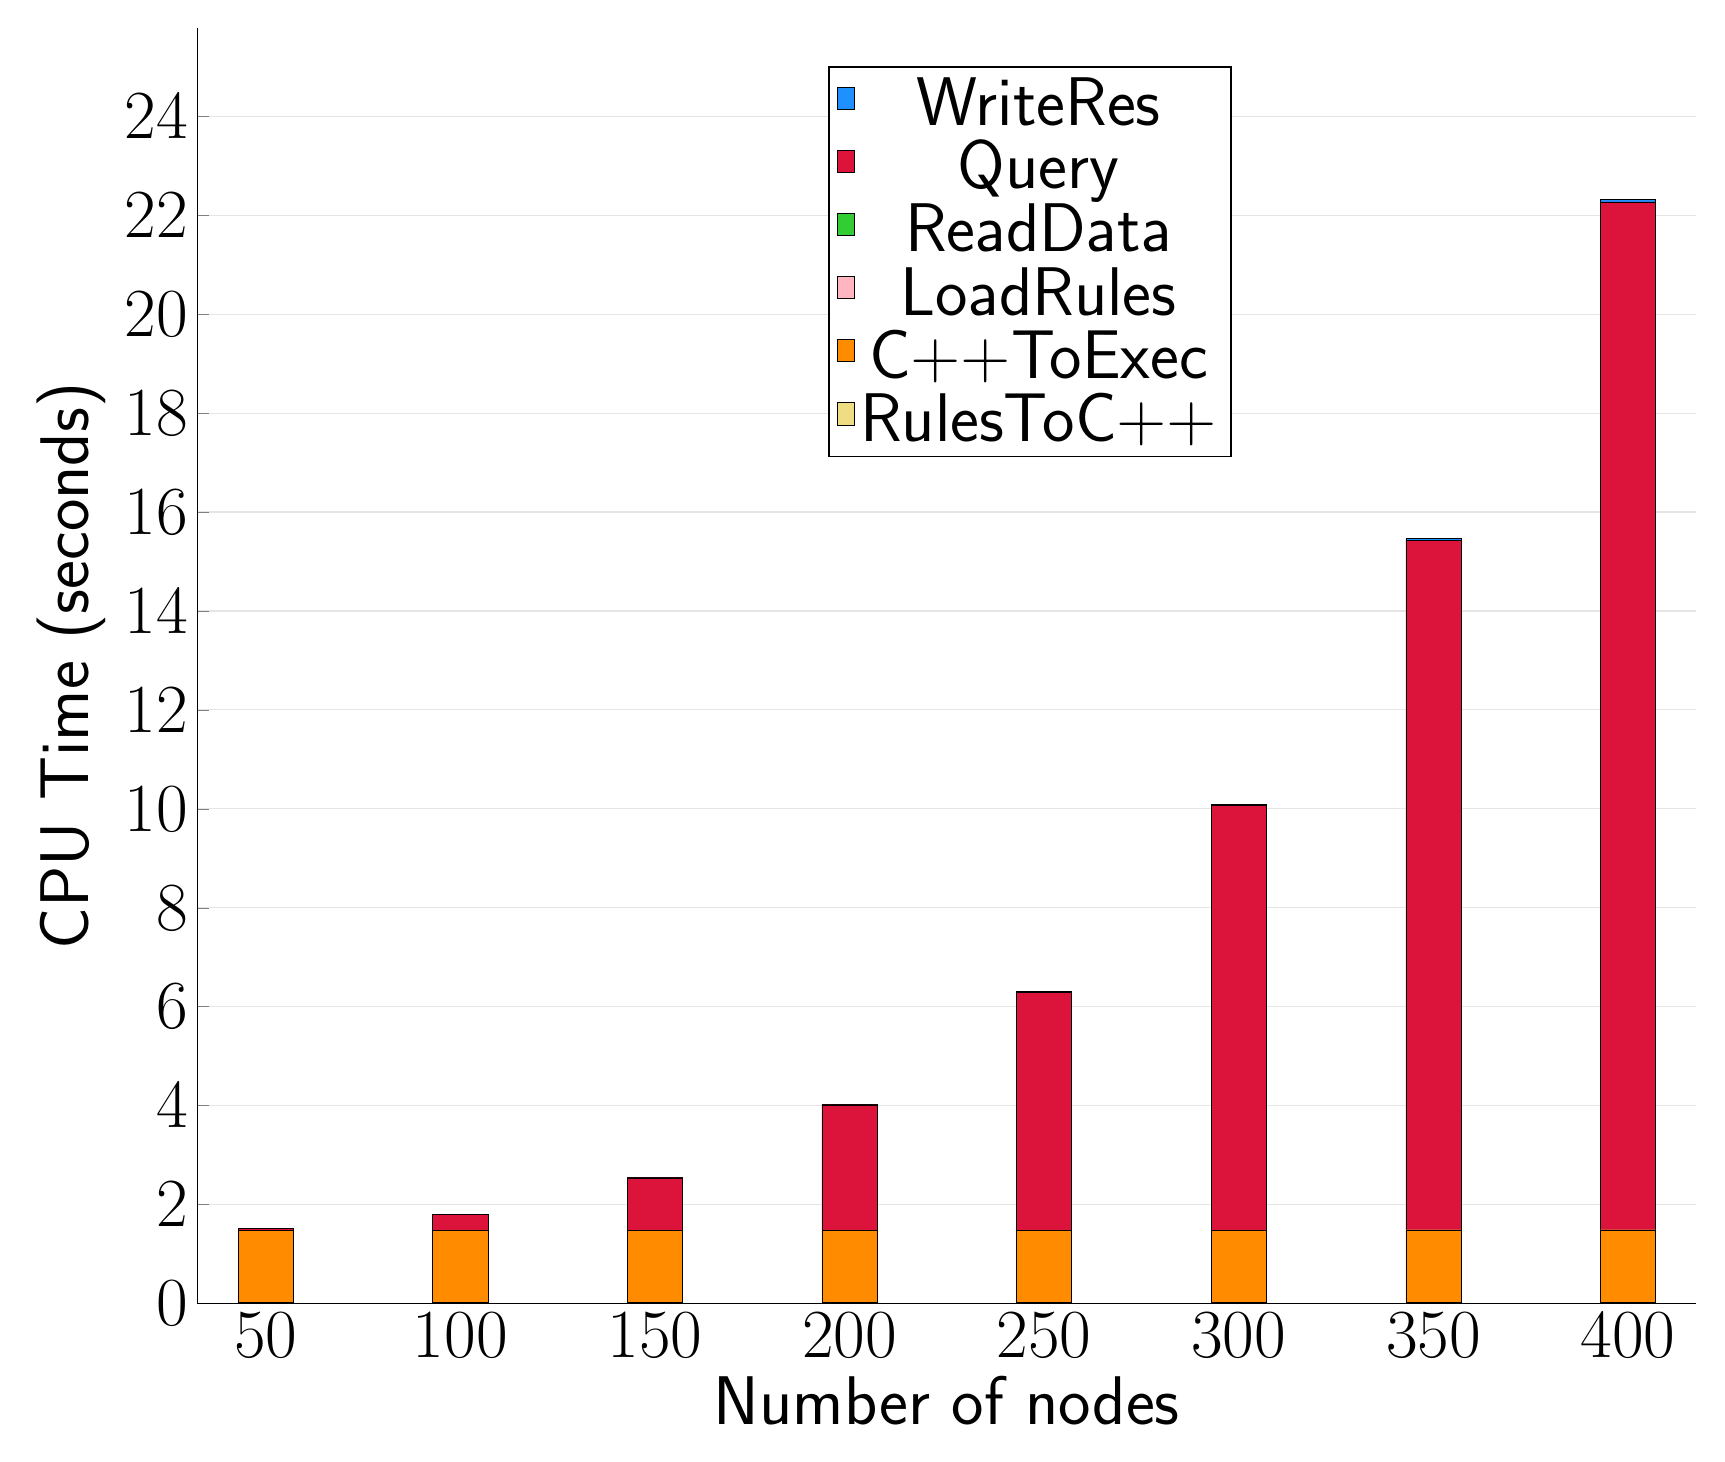
\begin{tikzpicture}
\begin{axis}[
   ybar stacked,
   width=1.7\textwidth,
   bar width=0.7cm,
   ymajorgrids, tick align=inside,
   major grid style={draw=gray!20},
   xtick=data,
   ymin=0, ymax=25.779619999999998,
   axis x line*=bottom,
   axis y line*=left,
   enlarge x limits=0.05,
   legend style={
       at={(0.69, 0.97)},
       anchor=north east,
       legend columns=1,
       font=\Huge,
   },
   ylabel={CPU Time (seconds)},
   xlabel={Number of nodes},
   label style={font=\Huge},
   tick label style={font=\Huge},
]
\addlegendimage{fill=DodgerBlue, draw=black, line width=0.2pt}
\addlegendentry{WriteRes}
\addlegendimage{fill=Crimson, draw=black, line width=0.2pt}
\addlegendentry{Query}
\addlegendimage{fill=LimeGreen, draw=black, line width=0.2pt}
\addlegendentry{ReadData}
\addlegendimage{fill=LightPink, draw=black, line width=0.2pt}
\addlegendentry{LoadRules}
\addlegendimage{fill=DarkOrange, draw=black, line width=0.2pt}
\addlegendentry{C++ToExec}
\addlegendimage{fill=LightGoldenrod, draw=black, line width=0.2pt}
\addlegendentry{RulesToC++}
\addplot +[fill=LightGoldenrod, draw=black, line width=0.2pt] coordinates {
(50, 0.030000000000000006)
(100, 0.030000000000000006)
(150, 0.030000000000000006)
(200, 0.030000000000000006)
(250, 0.030000000000000006)
(300, 0.030000000000000006)
(350, 0.030000000000000006)
(400, 0.030000000000000006)
};
\addplot +[fill=DarkOrange, draw=black, line width=0.2pt] coordinates {
(50, 1.4439999999999997)
(100, 1.4469999999999996)
(150, 1.4449999999999998)
(200, 1.4550000000000003)
(250, 1.4499999999999997)
(300, 1.457)
(350, 1.4600000000000002)
(400, 1.4580000000000002)
};
\addplot +[fill=LightPink, draw=black, line width=0.2pt] coordinates {
(50, 0.0001075)
(100, 0.00011080000000000001)
(150, 8.6e-05)
(200, 9.94e-05)
(250, 0.00012030000000000001)
(300, 9.63e-05)
(350, 0.00011220000000000002)
(400, 0.00011099999999999999)
};
\addplot +[fill=LimeGreen, draw=black, line width=0.2pt] coordinates {
(50, 0.0003652)
(100, 0.00045390000000000003)
(150, 0.0005567999999999999)
(200, 0.0006571999999999999)
(250, 0.0007957999999999999)
(300, 0.0007892000000000001)
(350, 0.0008537)
(400, 0.0009533)
};
\addplot +[fill=Crimson, draw=black, line width=0.2pt] coordinates {
(50, 0.0526721)
(100, 0.3230982)
(150, 1.066175)
(200, 2.532561)
(250, 4.815493)
(300, 8.581636)
(350, 13.94141)
(400, 20.779619999999998)
};
\addplot +[fill=DodgerBlue, draw=black, line width=0.2pt] coordinates {
(50, 0.0009512000000000001)
(100, 0.0030570000000000003)
(150, 0.0064953)
(200, 0.0115408)
(250, 0.0179507)
(300, 0.0255558)
(350, 0.0347213)
(400, 0.044857400000000006)
};
\end{axis}
\end{tikzpicture}

\end{document}
